\documentclass[]{article}
\usepackage{lmodern}
\usepackage{amssymb,amsmath}
\usepackage{ifxetex,ifluatex}
\usepackage{fixltx2e} % provides \textsubscript
\ifnum 0\ifxetex 1\fi\ifluatex 1\fi=0 % if pdftex
  \usepackage[T1]{fontenc}
  \usepackage[utf8]{inputenc}
\else % if luatex or xelatex
  \ifxetex
    \usepackage{mathspec}
  \else
    \usepackage{fontspec}
  \fi
  \defaultfontfeatures{Ligatures=TeX,Scale=MatchLowercase}
\fi
% use upquote if available, for straight quotes in verbatim environments
\IfFileExists{upquote.sty}{\usepackage{upquote}}{}
% use microtype if available
\IfFileExists{microtype.sty}{%
\usepackage{microtype}
\UseMicrotypeSet[protrusion]{basicmath} % disable protrusion for tt fonts
}{}
\usepackage[margin=1in]{geometry}
\usepackage{hyperref}
\hypersetup{unicode=true,
            pdftitle={Overfitting Analysis Mclust},
            pdfauthor={Renato Frey - renato.frey@unibas.ch},
            pdfborder={0 0 0},
            breaklinks=true}
\urlstyle{same}  % don't use monospace font for urls
\usepackage{color}
\usepackage{fancyvrb}
\newcommand{\VerbBar}{|}
\newcommand{\VERB}{\Verb[commandchars=\\\{\}]}
\DefineVerbatimEnvironment{Highlighting}{Verbatim}{commandchars=\\\{\}}
% Add ',fontsize=\small' for more characters per line
\usepackage{framed}
\definecolor{shadecolor}{RGB}{248,248,248}
\newenvironment{Shaded}{\begin{snugshade}}{\end{snugshade}}
\newcommand{\AlertTok}[1]{\textcolor[rgb]{0.94,0.16,0.16}{#1}}
\newcommand{\AnnotationTok}[1]{\textcolor[rgb]{0.56,0.35,0.01}{\textbf{\textit{#1}}}}
\newcommand{\AttributeTok}[1]{\textcolor[rgb]{0.77,0.63,0.00}{#1}}
\newcommand{\BaseNTok}[1]{\textcolor[rgb]{0.00,0.00,0.81}{#1}}
\newcommand{\BuiltInTok}[1]{#1}
\newcommand{\CharTok}[1]{\textcolor[rgb]{0.31,0.60,0.02}{#1}}
\newcommand{\CommentTok}[1]{\textcolor[rgb]{0.56,0.35,0.01}{\textit{#1}}}
\newcommand{\CommentVarTok}[1]{\textcolor[rgb]{0.56,0.35,0.01}{\textbf{\textit{#1}}}}
\newcommand{\ConstantTok}[1]{\textcolor[rgb]{0.00,0.00,0.00}{#1}}
\newcommand{\ControlFlowTok}[1]{\textcolor[rgb]{0.13,0.29,0.53}{\textbf{#1}}}
\newcommand{\DataTypeTok}[1]{\textcolor[rgb]{0.13,0.29,0.53}{#1}}
\newcommand{\DecValTok}[1]{\textcolor[rgb]{0.00,0.00,0.81}{#1}}
\newcommand{\DocumentationTok}[1]{\textcolor[rgb]{0.56,0.35,0.01}{\textbf{\textit{#1}}}}
\newcommand{\ErrorTok}[1]{\textcolor[rgb]{0.64,0.00,0.00}{\textbf{#1}}}
\newcommand{\ExtensionTok}[1]{#1}
\newcommand{\FloatTok}[1]{\textcolor[rgb]{0.00,0.00,0.81}{#1}}
\newcommand{\FunctionTok}[1]{\textcolor[rgb]{0.00,0.00,0.00}{#1}}
\newcommand{\ImportTok}[1]{#1}
\newcommand{\InformationTok}[1]{\textcolor[rgb]{0.56,0.35,0.01}{\textbf{\textit{#1}}}}
\newcommand{\KeywordTok}[1]{\textcolor[rgb]{0.13,0.29,0.53}{\textbf{#1}}}
\newcommand{\NormalTok}[1]{#1}
\newcommand{\OperatorTok}[1]{\textcolor[rgb]{0.81,0.36,0.00}{\textbf{#1}}}
\newcommand{\OtherTok}[1]{\textcolor[rgb]{0.56,0.35,0.01}{#1}}
\newcommand{\PreprocessorTok}[1]{\textcolor[rgb]{0.56,0.35,0.01}{\textit{#1}}}
\newcommand{\RegionMarkerTok}[1]{#1}
\newcommand{\SpecialCharTok}[1]{\textcolor[rgb]{0.00,0.00,0.00}{#1}}
\newcommand{\SpecialStringTok}[1]{\textcolor[rgb]{0.31,0.60,0.02}{#1}}
\newcommand{\StringTok}[1]{\textcolor[rgb]{0.31,0.60,0.02}{#1}}
\newcommand{\VariableTok}[1]{\textcolor[rgb]{0.00,0.00,0.00}{#1}}
\newcommand{\VerbatimStringTok}[1]{\textcolor[rgb]{0.31,0.60,0.02}{#1}}
\newcommand{\WarningTok}[1]{\textcolor[rgb]{0.56,0.35,0.01}{\textbf{\textit{#1}}}}
\usepackage{graphicx,grffile}
\makeatletter
\def\maxwidth{\ifdim\Gin@nat@width>\linewidth\linewidth\else\Gin@nat@width\fi}
\def\maxheight{\ifdim\Gin@nat@height>\textheight\textheight\else\Gin@nat@height\fi}
\makeatother
% Scale images if necessary, so that they will not overflow the page
% margins by default, and it is still possible to overwrite the defaults
% using explicit options in \includegraphics[width, height, ...]{}
\setkeys{Gin}{width=\maxwidth,height=\maxheight,keepaspectratio}
\IfFileExists{parskip.sty}{%
\usepackage{parskip}
}{% else
\setlength{\parindent}{0pt}
\setlength{\parskip}{6pt plus 2pt minus 1pt}
}
\setlength{\emergencystretch}{3em}  % prevent overfull lines
\providecommand{\tightlist}{%
  \setlength{\itemsep}{0pt}\setlength{\parskip}{0pt}}
\setcounter{secnumdepth}{0}
% Redefines (sub)paragraphs to behave more like sections
\ifx\paragraph\undefined\else
\let\oldparagraph\paragraph
\renewcommand{\paragraph}[1]{\oldparagraph{#1}\mbox{}}
\fi
\ifx\subparagraph\undefined\else
\let\oldsubparagraph\subparagraph
\renewcommand{\subparagraph}[1]{\oldsubparagraph{#1}\mbox{}}
\fi

%%% Use protect on footnotes to avoid problems with footnotes in titles
\let\rmarkdownfootnote\footnote%
\def\footnote{\protect\rmarkdownfootnote}

%%% Change title format to be more compact
\usepackage{titling}

% Create subtitle command for use in maketitle
\providecommand{\subtitle}[1]{
  \posttitle{
    \begin{center}\large#1\end{center}
    }
}

\setlength{\droptitle}{-2em}

  \title{Overfitting Analysis Mclust}
    \pretitle{\vspace{\droptitle}\centering\huge}
  \posttitle{\par}
    \author{Renato Frey -
\href{mailto:renato.frey@unibas.ch}{\nolinkurl{renato.frey@unibas.ch}}}
    \preauthor{\centering\large\emph}
  \postauthor{\par}
      \predate{\centering\large\emph}
  \postdate{\par}
    \date{12 June, 2019}


\begin{document}
\maketitle

Step 1: Generate 2d-dataset with two obvious clusters.

\begin{Shaded}
\begin{Highlighting}[]
\KeywordTok{set.seed}\NormalTok{(}\DecValTok{123}\NormalTok{)}

\NormalTok{m_x1 <-}\StringTok{ }\DecValTok{20}
\NormalTok{m_x2 <-}\StringTok{ }\DecValTok{25}
\NormalTok{m_y1 <-}\StringTok{ }\DecValTok{50}
\NormalTok{m_y2 <-}\StringTok{ }\DecValTok{80}
\NormalTok{means <-}\StringTok{ }\KeywordTok{data.frame}\NormalTok{(}\DataTypeTok{x=}\KeywordTok{c}\NormalTok{(m_x1, m_x2), }\DataTypeTok{y=}\KeywordTok{c}\NormalTok{(m_y1, m_y2))}

\NormalTok{x1 <-}\StringTok{ }\KeywordTok{sort}\NormalTok{(}\KeywordTok{rnorm}\NormalTok{(}\DecValTok{100}\NormalTok{, }\DataTypeTok{mean=}\NormalTok{m_x1, }\DataTypeTok{sd=}\DecValTok{1}\NormalTok{))}
\NormalTok{y1 <-}\StringTok{ }\KeywordTok{sort}\NormalTok{(}\KeywordTok{rnorm}\NormalTok{(}\DecValTok{100}\NormalTok{, }\DataTypeTok{mean=}\NormalTok{m_y1, }\DataTypeTok{sd=}\DecValTok{2}\NormalTok{))}
\NormalTok{ind1 <-}\StringTok{ }\KeywordTok{sample}\NormalTok{(}\DecValTok{1}\OperatorTok{:}\DecValTok{100}\NormalTok{, }\DecValTok{50}\NormalTok{)}
\NormalTok{ind2 <-}\StringTok{ }\KeywordTok{sample}\NormalTok{(}\DecValTok{1}\OperatorTok{:}\DecValTok{100}\NormalTok{, }\DecValTok{50}\NormalTok{)}
\NormalTok{y1[ind1] <-}\StringTok{ }\NormalTok{y1[ind2]}

\NormalTok{x2 <-}\StringTok{ }\KeywordTok{sort}\NormalTok{(}\KeywordTok{rnorm}\NormalTok{(}\DecValTok{100}\NormalTok{, }\DataTypeTok{mean=}\NormalTok{m_x2, }\DataTypeTok{sd=}\DecValTok{1}\NormalTok{))}
\NormalTok{y2 <-}\StringTok{ }\KeywordTok{sort}\NormalTok{(}\KeywordTok{rnorm}\NormalTok{(}\DecValTok{100}\NormalTok{, }\DataTypeTok{mean=}\NormalTok{m_y2, }\DataTypeTok{sd=}\DecValTok{3}\NormalTok{))}
\NormalTok{ind3 <-}\StringTok{ }\KeywordTok{sample}\NormalTok{(}\DecValTok{1}\OperatorTok{:}\DecValTok{100}\NormalTok{, }\DecValTok{50}\NormalTok{)}
\NormalTok{ind4 <-}\StringTok{ }\KeywordTok{sample}\NormalTok{(}\DecValTok{1}\OperatorTok{:}\DecValTok{100}\NormalTok{, }\DecValTok{50}\NormalTok{)}
\NormalTok{y2[ind3] <-}\StringTok{ }\NormalTok{y2[ind4]}

\NormalTok{x <-}\StringTok{ }\KeywordTok{c}\NormalTok{(x1, x2)}
\NormalTok{y <-}\StringTok{ }\KeywordTok{c}\NormalTok{(y1, y2)}
\NormalTok{d <-}\StringTok{ }\KeywordTok{cbind}\NormalTok{(x,y)}
\KeywordTok{write.csv}\NormalTok{(d, }\DataTypeTok{file=}\StringTok{"simdat.csv"}\NormalTok{)}

\KeywordTok{par}\NormalTok{(}\DataTypeTok{mar=}\KeywordTok{c}\NormalTok{(}\DecValTok{4}\NormalTok{,}\DecValTok{3}\NormalTok{,}\DecValTok{3}\NormalTok{,}\DecValTok{1}\NormalTok{))}
\KeywordTok{plot}\NormalTok{(d, }\DataTypeTok{las=}\DecValTok{1}\NormalTok{, }\DataTypeTok{pch=}\DecValTok{16}\NormalTok{, }\DataTypeTok{cex=}\NormalTok{.}\DecValTok{7}\NormalTok{, }\DataTypeTok{main=}\StringTok{"Dataset with cluster means"}\NormalTok{)}
\KeywordTok{points}\NormalTok{(means, }\DataTypeTok{pch=}\DecValTok{15}\NormalTok{, }\DataTypeTok{cex=}\FloatTok{1.2}\NormalTok{, }\DataTypeTok{col=}\StringTok{"red"}\NormalTok{)}
\end{Highlighting}
\end{Shaded}

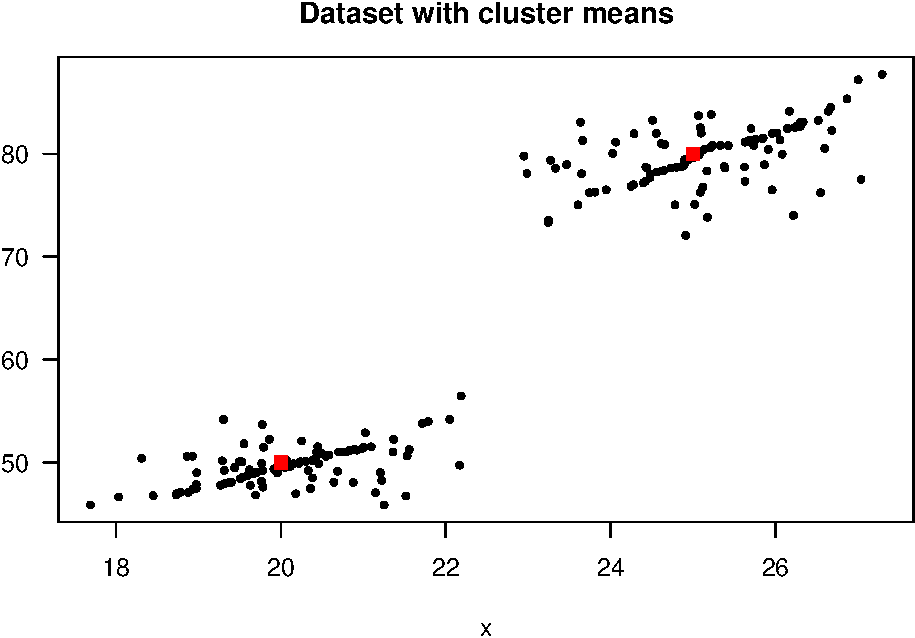
\includegraphics{mclust_sim_files/figure-latex/unnamed-chunk-1-1.pdf}

Step 2: Use Mclust to fit three different GMMs.

\begin{Shaded}
\begin{Highlighting}[]
\KeywordTok{library}\NormalTok{(mclust)}
\end{Highlighting}
\end{Shaded}

\begin{verbatim}
## Package 'mclust' version 5.4.3
## Type 'citation("mclust")' for citing this R package in publications.
\end{verbatim}

\begin{Shaded}
\begin{Highlighting}[]
\NormalTok{m1 <-}\StringTok{ }\KeywordTok{Mclust}\NormalTok{(d, }\DataTypeTok{G=}\DecValTok{1}\OperatorTok{:}\DecValTok{10}\NormalTok{)}
\NormalTok{m2 <-}\StringTok{ }\KeywordTok{Mclust}\NormalTok{(d, }\DataTypeTok{G=}\DecValTok{1}\OperatorTok{:}\DecValTok{10}\NormalTok{, }\DataTypeTok{modelNames=}\KeywordTok{c}\NormalTok{(}\StringTok{"EEE"}\NormalTok{))}
\NormalTok{m3 <-}\StringTok{ }\KeywordTok{Mclust}\NormalTok{(d, }\DataTypeTok{G=}\DecValTok{1}\OperatorTok{:}\DecValTok{10}\NormalTok{, }\DataTypeTok{modelNames=}\KeywordTok{c}\NormalTok{(}\StringTok{"EEV"}\NormalTok{))}

\CommentTok{# save the cluster means}
\NormalTok{cmeans_m1 <-}\StringTok{ }\KeywordTok{t}\NormalTok{(}\KeywordTok{summary}\NormalTok{(m1)}\OperatorTok{$}\NormalTok{mean)}
\NormalTok{cmeans_m2 <-}\StringTok{ }\KeywordTok{t}\NormalTok{(}\KeywordTok{summary}\NormalTok{(m2)}\OperatorTok{$}\NormalTok{mean)}
\NormalTok{cmeans_m3 <-}\StringTok{ }\KeywordTok{t}\NormalTok{(}\KeywordTok{summary}\NormalTok{(m3)}\OperatorTok{$}\NormalTok{mean)}

\ControlFlowTok{for}\NormalTok{ (i }\ControlFlowTok{in} \DecValTok{1}\OperatorTok{:}\DecValTok{3}\NormalTok{) \{}
  \KeywordTok{plot}\NormalTok{(}\KeywordTok{get}\NormalTok{(}\KeywordTok{paste}\NormalTok{(}\StringTok{"m"}\NormalTok{, i, }\DataTypeTok{sep=}\StringTok{""}\NormalTok{)), }\DataTypeTok{what=}\StringTok{"classification"}\NormalTok{)}
  \KeywordTok{title}\NormalTok{(}\KeywordTok{paste}\NormalTok{(}\StringTok{"Classification according to model"}\NormalTok{, i))}
\NormalTok{\}}
\end{Highlighting}
\end{Shaded}

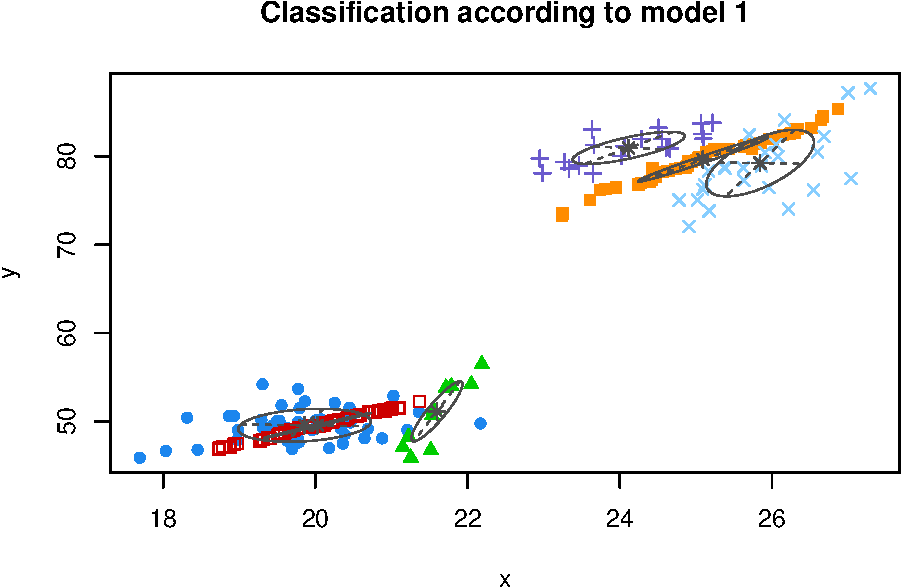
\includegraphics{mclust_sim_files/figure-latex/unnamed-chunk-2-1.pdf}
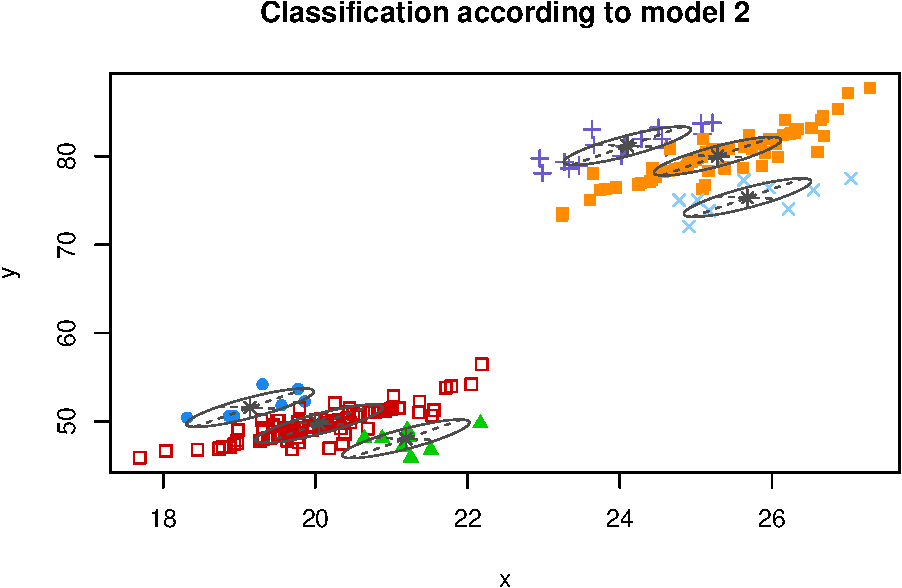
\includegraphics{mclust_sim_files/figure-latex/unnamed-chunk-2-2.pdf}
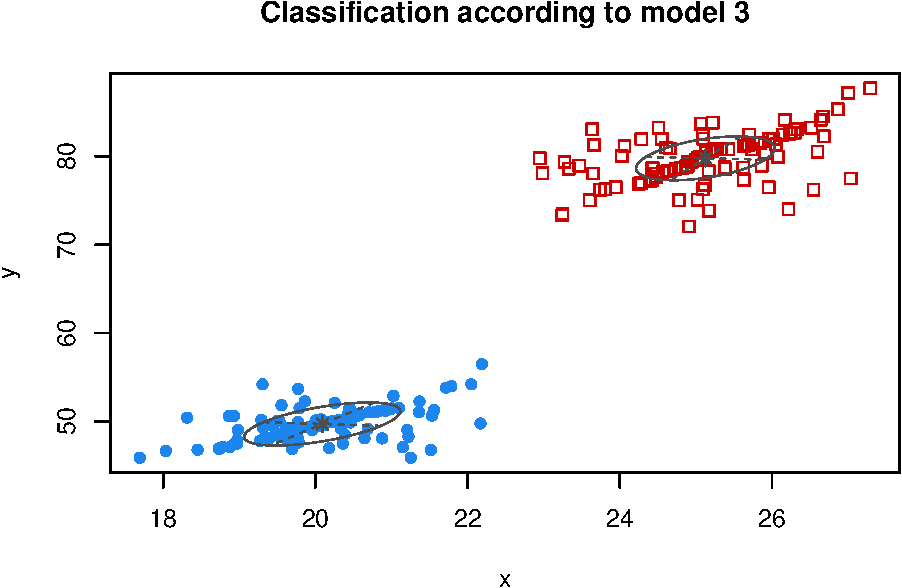
\includegraphics{mclust_sim_files/figure-latex/unnamed-chunk-2-3.pdf}

For models 1 and 2, the plots above show that too many clusters are
estimated, with several cluster means being very close to each other
(small euclidean distance between cluster means).

Step 3: Use a Gaussian kernel to estimate the empirical density in the
dataset.

\begin{Shaded}
\begin{Highlighting}[]
\KeywordTok{library}\NormalTok{(ks)}
\NormalTok{dens <-}\StringTok{ }\KeywordTok{kde}\NormalTok{(d, }\DataTypeTok{binned=}\NormalTok{F)}

\CommentTok{# save the points where the density was evaluated (will be needed below)}
\NormalTok{evalp <-}\StringTok{ }\KeywordTok{expand.grid}\NormalTok{(dens}\OperatorTok{$}\NormalTok{eval.points[[}\DecValTok{1}\NormalTok{]], dens}\OperatorTok{$}\NormalTok{eval.points[[}\DecValTok{2}\NormalTok{]])}
\KeywordTok{colnames}\NormalTok{(evalp) <-}\StringTok{ }\KeywordTok{c}\NormalTok{(}\StringTok{"x"}\NormalTok{, }\StringTok{"y"}\NormalTok{)}

\CommentTok{# predict the density at the cluster means}
\NormalTok{dens_cmeans_m1 <-}\StringTok{ }\KeywordTok{predict}\NormalTok{(dens, }\DataTypeTok{x=}\NormalTok{cmeans_m1)}
\NormalTok{dens_cmeans_m2 <-}\StringTok{ }\KeywordTok{predict}\NormalTok{(dens, }\DataTypeTok{x=}\NormalTok{cmeans_m2)}
\NormalTok{dens_cmeans_m3 <-}\StringTok{ }\KeywordTok{predict}\NormalTok{(dens, }\DataTypeTok{x=}\NormalTok{cmeans_m3)}

\CommentTok{# plot the empirical density and add the cluster means}
\ControlFlowTok{for}\NormalTok{ (i }\ControlFlowTok{in} \DecValTok{1}\OperatorTok{:}\DecValTok{3}\NormalTok{) \{}
  \KeywordTok{plot}\NormalTok{(dens, }\DataTypeTok{display=}\StringTok{"image"}\NormalTok{, }\DataTypeTok{las=}\DecValTok{1}\NormalTok{,}
       \DataTypeTok{main=}\KeywordTok{paste}\NormalTok{(}\StringTok{"Empirical density of data with cluster means of model"}\NormalTok{, i))}
  \KeywordTok{points}\NormalTok{(d, }\DataTypeTok{pch=}\DecValTok{16}\NormalTok{, }\DataTypeTok{cex=}\FloatTok{0.3}\NormalTok{, }\DataTypeTok{col=}\StringTok{"black"}\NormalTok{)}
\NormalTok{  myconts <-}\StringTok{ }\KeywordTok{round}\NormalTok{(}\KeywordTok{seq}\NormalTok{(}\FloatTok{0.0001}\NormalTok{, }\KeywordTok{max}\NormalTok{(dens}\OperatorTok{$}\NormalTok{estimate), }\DataTypeTok{length.out=}\DecValTok{8}\NormalTok{), }\DecValTok{2}\NormalTok{)}
  \KeywordTok{plot}\NormalTok{(dens, }\DataTypeTok{col=}\StringTok{"black"}\NormalTok{, }\DataTypeTok{add=}\NormalTok{T, }\DataTypeTok{abs.cont=}\NormalTok{myconts)}
  \KeywordTok{points}\NormalTok{(}\KeywordTok{get}\NormalTok{(}\KeywordTok{paste}\NormalTok{(}\StringTok{"cmeans_m"}\NormalTok{, i, }\DataTypeTok{sep=}\StringTok{""}\NormalTok{)), }\DataTypeTok{col=}\StringTok{"cyan"}\NormalTok{, }\DataTypeTok{pch=}\DecValTok{16}\NormalTok{, }\DataTypeTok{cex=}\FloatTok{1.5}\NormalTok{)}
\NormalTok{\}}
\end{Highlighting}
\end{Shaded}

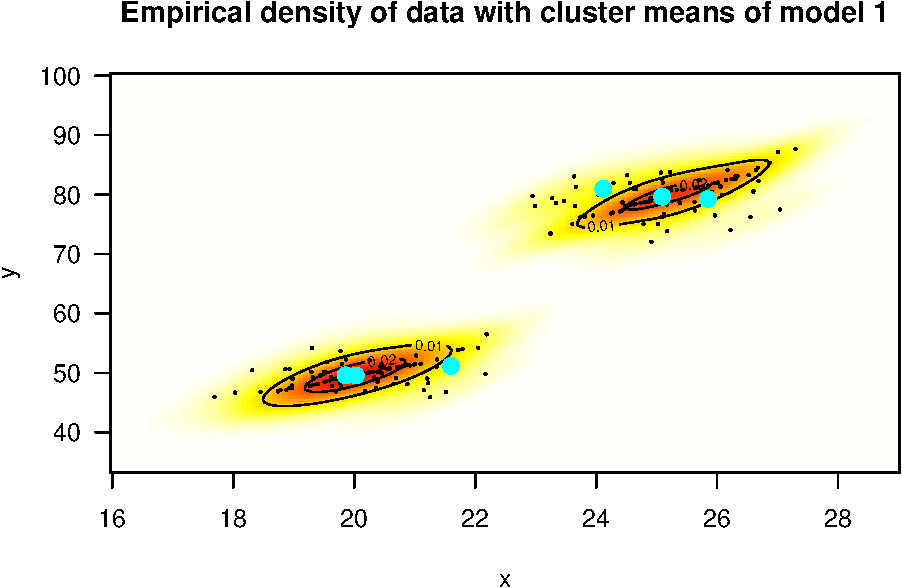
\includegraphics{mclust_sim_files/figure-latex/unnamed-chunk-3-1.pdf}
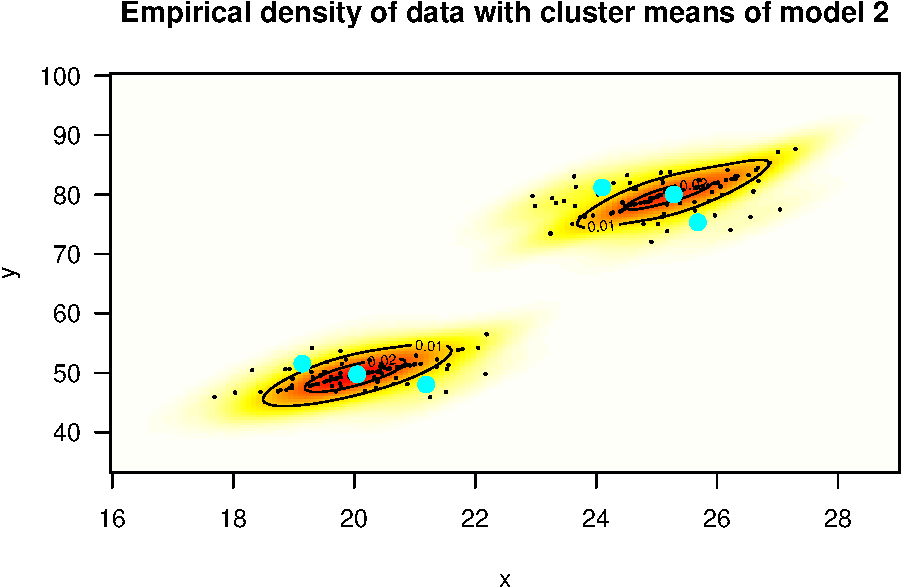
\includegraphics{mclust_sim_files/figure-latex/unnamed-chunk-3-2.pdf}
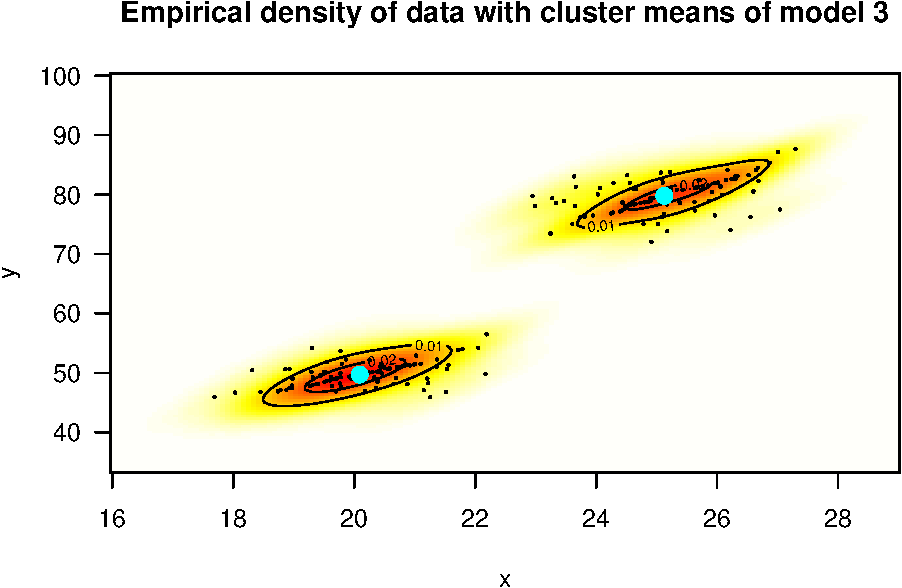
\includegraphics{mclust_sim_files/figure-latex/unnamed-chunk-3-3.pdf}

Step 4: Generate a null-model to estimate the ``saturation'' of the
identified clusters: specifically, shuffle the dataset 100 times (by
column, that is, keeping the marginal distributions of each variable
constant, but removing any clusters).

\begin{Shaded}
\begin{Highlighting}[]
\NormalTok{null_m1 <-}\StringTok{ }\OtherTok{NULL}
\NormalTok{null_m2 <-}\StringTok{ }\OtherTok{NULL}
\NormalTok{null_m3 <-}\StringTok{ }\OtherTok{NULL}
\NormalTok{null_model_z <-}\StringTok{ }\OtherTok{NULL}
\ControlFlowTok{for}\NormalTok{ (i }\ControlFlowTok{in} \DecValTok{1}\OperatorTok{:}\DecValTok{100}\NormalTok{) \{}

  \CommentTok{# shuffle dataset}
\NormalTok{  d_shf <-}\StringTok{ }\KeywordTok{apply}\NormalTok{(d, }\DecValTok{2}\NormalTok{, sample)}
  
  \CommentTok{# estimate density}
\NormalTok{  dens_shf <-}\StringTok{ }\KeywordTok{kde}\NormalTok{(d_shf, }\DataTypeTok{binned=}\NormalTok{F)}
  
  \CommentTok{# get (and store) the density at the cluster centers}
\NormalTok{  shf_cmeans_m1 <-}\StringTok{ }\KeywordTok{predict}\NormalTok{(dens_shf, }\DataTypeTok{x=}\NormalTok{cmeans_m1)}
\NormalTok{  null_m1 <-}\StringTok{ }\KeywordTok{rbind}\NormalTok{(null_m1, shf_cmeans_m1)}
  
\NormalTok{  shf_cmeans_m2 <-}\StringTok{ }\KeywordTok{predict}\NormalTok{(dens_shf, }\DataTypeTok{x=}\NormalTok{cmeans_m2)}
\NormalTok{  null_m2 <-}\StringTok{ }\KeywordTok{rbind}\NormalTok{(null_m2, shf_cmeans_m2)}
  
\NormalTok{  shf_cmeans_m3 <-}\StringTok{ }\KeywordTok{predict}\NormalTok{(dens_shf, }\DataTypeTok{x=}\NormalTok{cmeans_m3)}
\NormalTok{  null_m3 <-}\StringTok{ }\KeywordTok{rbind}\NormalTok{(null_m3, shf_cmeans_m3)}
  
  \CommentTok{# get (and store) the density at each actual datapoint}
\NormalTok{  shf_z <-}\StringTok{ }\KeywordTok{predict}\NormalTok{(dens_shf, }\DataTypeTok{x=}\NormalTok{evalp)}
\NormalTok{  null_model_z <-}\StringTok{ }\KeywordTok{rbind}\NormalTok{(null_model_z, shf_z)}
\NormalTok{\}}
\end{Highlighting}
\end{Shaded}

Step 5: Determine a ``non-parametric'' p-value for each cluster, that
is, the proportion of simulation runs in which the density at the
cluster centers were LARGER (under the null-model) than the density of
the clusters centers in the actual dataset

\begin{Shaded}
\begin{Highlighting}[]
\NormalTok{pvals_m1 <-}\StringTok{ }\KeywordTok{rowMeans}\NormalTok{(}\KeywordTok{apply}\NormalTok{(null_m1, }\DecValTok{1}\NormalTok{, }\ControlFlowTok{function}\NormalTok{(x) \{x }\OperatorTok{>}\StringTok{ }\NormalTok{dens_cmeans_m1\}))}
\NormalTok{pvals_m2 <-}\StringTok{ }\KeywordTok{rowMeans}\NormalTok{(}\KeywordTok{apply}\NormalTok{(null_m2, }\DecValTok{1}\NormalTok{, }\ControlFlowTok{function}\NormalTok{(x) \{x }\OperatorTok{>}\StringTok{ }\NormalTok{dens_cmeans_m2\}))}
\NormalTok{pvals_m3 <-}\StringTok{ }\KeywordTok{rowMeans}\NormalTok{(}\KeywordTok{apply}\NormalTok{(null_m3, }\DecValTok{1}\NormalTok{, }\ControlFlowTok{function}\NormalTok{(x) \{x }\OperatorTok{>}\StringTok{ }\NormalTok{dens_cmeans_m3\}))}
\KeywordTok{print}\NormalTok{(pvals_m1)}
\end{Highlighting}
\end{Shaded}

\begin{verbatim}
## [1] 0.00 0.00 0.00 0.07 0.00 0.00
\end{verbatim}

\begin{Shaded}
\begin{Highlighting}[]
\KeywordTok{print}\NormalTok{(pvals_m2)}
\end{Highlighting}
\end{Shaded}

\begin{verbatim}
## [1] 0.80 0.00 0.75 0.12 0.00 0.96
\end{verbatim}

\begin{Shaded}
\begin{Highlighting}[]
\KeywordTok{print}\NormalTok{(pvals_m3)}
\end{Highlighting}
\end{Shaded}

\begin{verbatim}
## [1] 0 0
\end{verbatim}

\begin{Shaded}
\begin{Highlighting}[]
\CommentTok{# get the average density across all the shuffled datasets (i.e., the null-model)}
\NormalTok{tmp <-}\StringTok{ }\KeywordTok{colMeans}\NormalTok{(null_model_z)}
\NormalTok{xs <-}\StringTok{ }\KeywordTok{unique}\NormalTok{(evalp}\OperatorTok{$}\NormalTok{x)}
\NormalTok{ys <-}\StringTok{ }\KeywordTok{unique}\NormalTok{(evalp}\OperatorTok{$}\NormalTok{y)}
\NormalTok{out <-}\StringTok{ }\KeywordTok{as.data.frame}\NormalTok{(}\KeywordTok{matrix}\NormalTok{(}\OtherTok{NA}\NormalTok{, }\DataTypeTok{nrow=}\KeywordTok{length}\NormalTok{(xs), }\DataTypeTok{ncol=}\KeywordTok{length}\NormalTok{(ys)))}
\KeywordTok{rownames}\NormalTok{(out) <-}\StringTok{ }\NormalTok{xs}
\KeywordTok{colnames}\NormalTok{(out) <-}\StringTok{ }\NormalTok{ys}
\ControlFlowTok{for}\NormalTok{ (k }\ControlFlowTok{in} \DecValTok{1}\OperatorTok{:}\KeywordTok{length}\NormalTok{(tmp)) \{}
\NormalTok{  out[}\KeywordTok{as.character}\NormalTok{(evalp}\OperatorTok{$}\NormalTok{x[k]), }\KeywordTok{as.character}\NormalTok{(evalp}\OperatorTok{$}\NormalTok{y[k])] <-}\StringTok{ }\NormalTok{tmp[k]}
\NormalTok{\}}

\CommentTok{# plot the average density add p-values to each of the cluster means}
\ControlFlowTok{for}\NormalTok{ (i }\ControlFlowTok{in} \DecValTok{1}\OperatorTok{:}\DecValTok{3}\NormalTok{) \{}
  \KeywordTok{image}\NormalTok{(}\DataTypeTok{x=}\NormalTok{xs, }\DataTypeTok{y=}\NormalTok{ys, }\DataTypeTok{z=}\DecValTok{1}\OperatorTok{-}\KeywordTok{as.matrix}\NormalTok{(out), }\DataTypeTok{las=}\DecValTok{1}\NormalTok{, }\DataTypeTok{xlab=}\StringTok{"x"}\NormalTok{, }\DataTypeTok{ylab=}\StringTok{"y"}\NormalTok{,}
        \DataTypeTok{main=}\KeywordTok{paste}\NormalTok{(}\StringTok{"Density of null model with cluster means / p-values of model"}\NormalTok{, i))}
  \KeywordTok{points}\NormalTok{(d, }\DataTypeTok{pch=}\DecValTok{16}\NormalTok{, }\DataTypeTok{cex=}\FloatTok{0.3}\NormalTok{, }\DataTypeTok{col=}\StringTok{"black"}\NormalTok{)}
  \KeywordTok{plot}\NormalTok{(dens, }\DataTypeTok{col=}\StringTok{"black"}\NormalTok{, }\DataTypeTok{add=}\NormalTok{T, }\DataTypeTok{abs.cont=}\NormalTok{myconts)}
  \KeywordTok{points}\NormalTok{(}\KeywordTok{get}\NormalTok{(}\KeywordTok{paste}\NormalTok{(}\StringTok{"cmeans_m"}\NormalTok{, i, }\DataTypeTok{sep=}\StringTok{""}\NormalTok{)), }\DataTypeTok{col=}\StringTok{"cyan"}\NormalTok{, }\DataTypeTok{pch=}\DecValTok{16}\NormalTok{, }\DataTypeTok{cex=}\FloatTok{1.5}\NormalTok{)}
  \KeywordTok{text}\NormalTok{(}\KeywordTok{round}\NormalTok{(}\KeywordTok{get}\NormalTok{(}\KeywordTok{paste}\NormalTok{(}\StringTok{"pvals_m"}\NormalTok{, i, }\DataTypeTok{sep=}\StringTok{""}\NormalTok{)), }\DecValTok{2}\NormalTok{),}
       \DataTypeTok{x=}\KeywordTok{get}\NormalTok{(}\KeywordTok{paste}\NormalTok{(}\StringTok{"cmeans_m"}\NormalTok{, i, }\DataTypeTok{sep=}\StringTok{""}\NormalTok{))[,}\DecValTok{1}\NormalTok{],}
       \DataTypeTok{y=}\KeywordTok{get}\NormalTok{(}\KeywordTok{paste}\NormalTok{(}\StringTok{"cmeans_m"}\NormalTok{, i, }\DataTypeTok{sep=}\StringTok{""}\NormalTok{))[,}\DecValTok{2}\NormalTok{], }\DataTypeTok{cex=}\NormalTok{.}\DecValTok{7}\NormalTok{)}
\NormalTok{\}}
\end{Highlighting}
\end{Shaded}

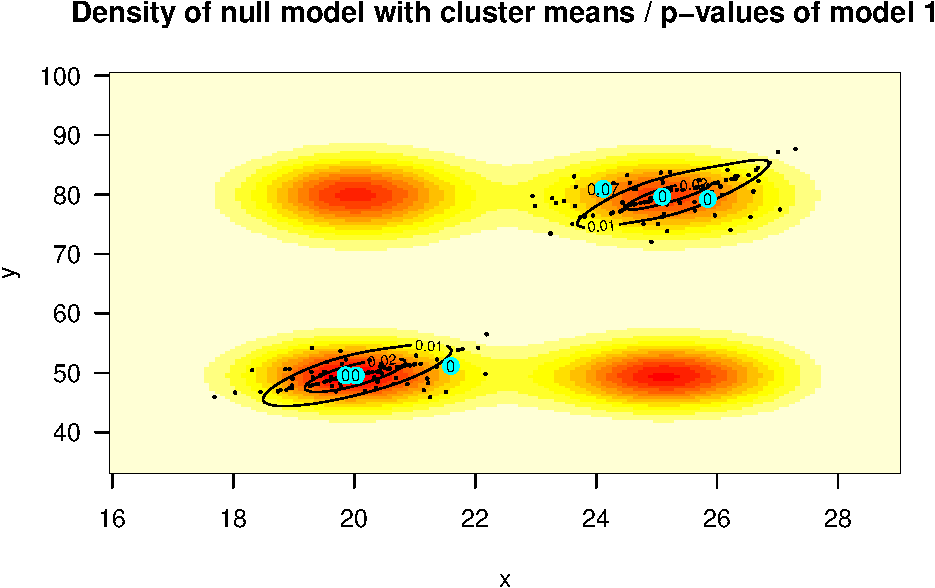
\includegraphics{mclust_sim_files/figure-latex/unnamed-chunk-5-1.pdf}
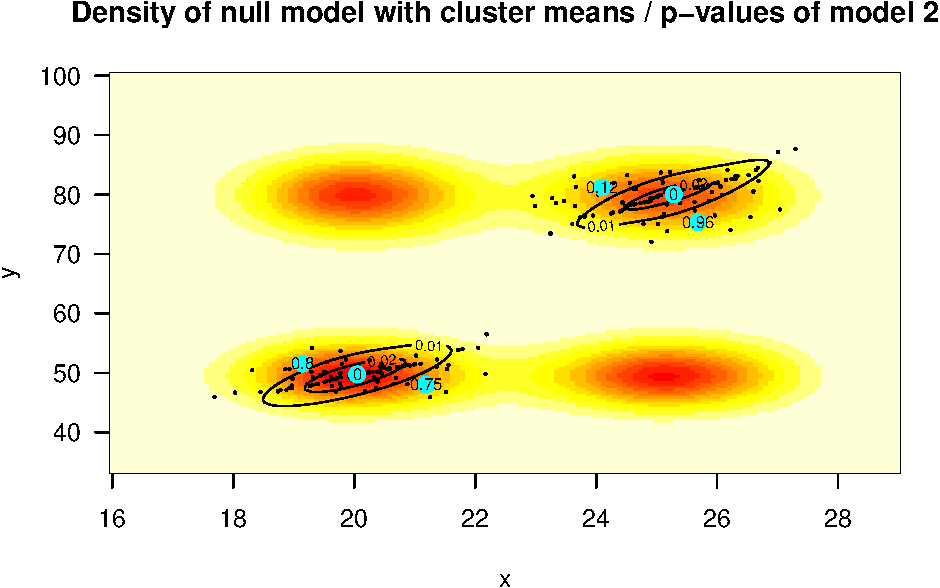
\includegraphics{mclust_sim_files/figure-latex/unnamed-chunk-5-2.pdf}
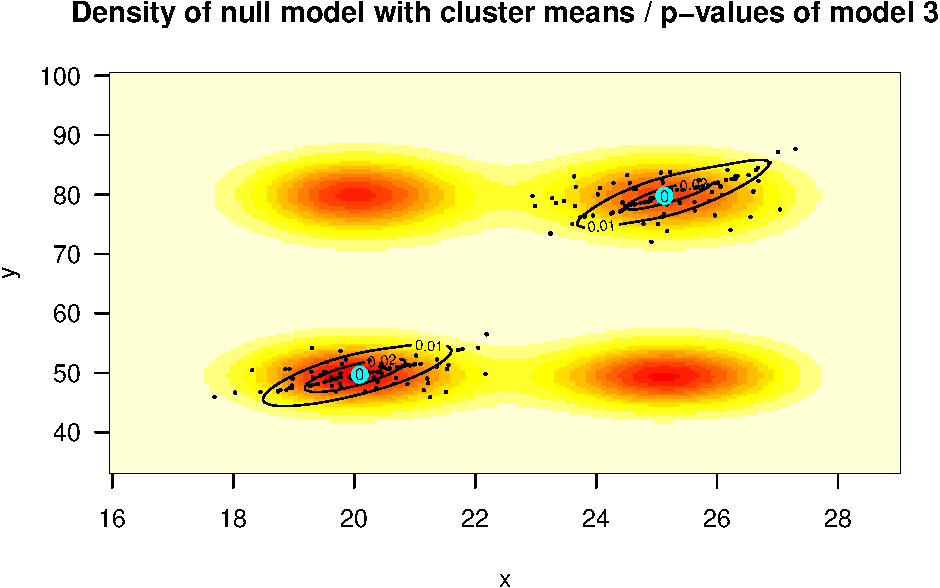
\includegraphics{mclust_sim_files/figure-latex/unnamed-chunk-5-3.pdf}

Interim conclusions:

For model 1 this saturation analysis does not recognize that there exist
several spurious clusters, because most of them happen to have means
right at the peaks of the empirical density.

For model 2, this analysis works because some of the spurious clusters
have means slightly outside the peaks of the empirical density, that is,
where the density under the null-model peaks ``higher'' sufficiently
often.

For model 3, the two cluster means are at the peaks of the empirical
density, thus correctly resulting in very small p-values.

We next estimate a variational Bayesian gaussian mixture model, as
obtained from using the Python-package scikit-learn (the following code
illustrates the key steps in Python):

\begin{Shaded}
\begin{Highlighting}[]
\NormalTok{  import sklearn.mixture as sklm}
\NormalTok{  gmm =}\StringTok{ }\KeywordTok{sklm.BayesianGaussianMixture}\NormalTok{(}\DataTypeTok{n_components =} \DecValTok{10}\NormalTok{,}
                                     \DataTypeTok{n_init =} \DecValTok{5}\NormalTok{,}
                                     \DataTypeTok{covariance_type =} \StringTok{'full'}\NormalTok{)}
\NormalTok{  c_means =}\StringTok{ }\NormalTok{gmm.means_}
\NormalTok{  c_cov =}\StringTok{ }\NormalTok{gmm.covariances_}
\NormalTok{  c_weights =}\StringTok{ }\NormalTok{gmm.weights_}
\NormalTok{  likelihood =}\StringTok{ }\NormalTok{gmm.lower_bound_}
\end{Highlighting}
\end{Shaded}

The following code reads in and visualizes the identified clusters:

\begin{Shaded}
\begin{Highlighting}[]
\KeywordTok{plot}\NormalTok{(d, }\DataTypeTok{las=}\DecValTok{1}\NormalTok{, }\DataTypeTok{pch=}\DecValTok{16}\NormalTok{, }\DataTypeTok{cex=}\NormalTok{.}\DecValTok{7}\NormalTok{, }\DataTypeTok{main=}\StringTok{"Dataset with Bayesian GMM."}\NormalTok{)}
\KeywordTok{points}\NormalTok{(means, }\DataTypeTok{pch=}\DecValTok{15}\NormalTok{, }\DataTypeTok{cex=}\FloatTok{1.2}\NormalTok{, }\DataTypeTok{col=}\StringTok{"red"}\NormalTok{)}

\CommentTok{# read values from BayesianGaussianMixture (scikit-learn)}
\NormalTok{means <-}\StringTok{ }\KeywordTok{read.csv}\NormalTok{(}\StringTok{"../python/gmm/out/means.csv"}\NormalTok{, }\DataTypeTok{header=}\NormalTok{F)}
\NormalTok{weights <-}\StringTok{ }\KeywordTok{unlist}\NormalTok{(}\KeywordTok{read.csv}\NormalTok{(}\StringTok{"../python/gmm/out/weights.csv"}\NormalTok{, }\DataTypeTok{header=}\NormalTok{F))}
\KeywordTok{print}\NormalTok{(}\KeywordTok{round}\NormalTok{(weights, }\DecValTok{4}\NormalTok{))}
\end{Highlighting}
\end{Shaded}

\begin{verbatim}
##    V11    V12    V13    V14    V15    V16    V17    V18    V19   V110 
## 0.5022 0.4973 0.0004 0.0000 0.0000 0.0000 0.0000 0.0000 0.0000 0.0000
\end{verbatim}

\begin{Shaded}
\begin{Highlighting}[]
\CommentTok{# add constant to visualize all clusters (even the ones we really small weights)}
\NormalTok{weights <-}\StringTok{ }\NormalTok{weights }\OperatorTok{+}\StringTok{ }\FloatTok{.04}
\NormalTok{weights <-}\StringTok{ }\NormalTok{weights }\OperatorTok{/}\StringTok{ }\KeywordTok{max}\NormalTok{(weights) }\OperatorTok{*}\StringTok{ }\FloatTok{.2}

\ControlFlowTok{if}\NormalTok{ (T) \{}
\NormalTok{  means[}\DecValTok{3}\OperatorTok{:}\DecValTok{10}\NormalTok{,}\DecValTok{1}\NormalTok{] <-}\StringTok{ }\NormalTok{means[}\DecValTok{3}\OperatorTok{:}\DecValTok{10}\NormalTok{,}\DecValTok{1}\NormalTok{] }\OperatorTok{+}\StringTok{ }\KeywordTok{runif}\NormalTok{(}\DecValTok{8}\NormalTok{, }\DataTypeTok{min=}\OperatorTok{-}\NormalTok{.}\DecValTok{5}\NormalTok{, }\DataTypeTok{max=}\NormalTok{.}\DecValTok{5}\NormalTok{)}
\NormalTok{  means[}\DecValTok{3}\OperatorTok{:}\DecValTok{10}\NormalTok{,}\DecValTok{2}\NormalTok{] <-}\StringTok{ }\NormalTok{means[}\DecValTok{3}\OperatorTok{:}\DecValTok{10}\NormalTok{,}\DecValTok{2}\NormalTok{] }\OperatorTok{+}\StringTok{ }\KeywordTok{runif}\NormalTok{(}\DecValTok{8}\NormalTok{, }\DataTypeTok{min=}\OperatorTok{-}\NormalTok{.}\DecValTok{5}\NormalTok{, }\DataTypeTok{max=}\NormalTok{.}\DecValTok{5}\NormalTok{)}
\NormalTok{\}}

\ControlFlowTok{for}\NormalTok{ (i }\ControlFlowTok{in} \DecValTok{1}\OperatorTok{:}\KeywordTok{nrow}\NormalTok{(means)) \{}
\NormalTok{  covars <-}\StringTok{ }\KeywordTok{read.csv}\NormalTok{(}\KeywordTok{paste}\NormalTok{(}\StringTok{"../python/gmm/out/covars_c"}\NormalTok{, i}\DecValTok{-1}\NormalTok{, }\StringTok{".csv"}\NormalTok{, }\DataTypeTok{sep=}\StringTok{""}\NormalTok{),}
                     \DataTypeTok{header=}\NormalTok{F)}

\NormalTok{  m <-}\StringTok{ }\KeywordTok{as.numeric}\NormalTok{(means[i,])}
\NormalTok{  c <-}\StringTok{ }\KeywordTok{matrix}\NormalTok{(}\KeywordTok{rev}\NormalTok{(}\KeywordTok{unlist}\NormalTok{(covars)), }\DataTypeTok{nrow=}\KeywordTok{nrow}\NormalTok{(covars))}
  
\NormalTok{  e <-}\StringTok{ }\KeywordTok{eigen}\NormalTok{(c)}
\NormalTok{  eig_vecs <-}\StringTok{ }\NormalTok{e}\OperatorTok{$}\NormalTok{vectors}
\NormalTok{  unit_eig_vec <-}\StringTok{ }\NormalTok{eig_vecs[,}\DecValTok{2}\NormalTok{] }\CommentTok{#/ norm(eig_vecs)}
\NormalTok{  angle <-}\StringTok{ }\KeywordTok{atan2}\NormalTok{(unit_eig_vec[}\DecValTok{2}\NormalTok{], unit_eig_vec[}\DecValTok{1}\NormalTok{])}
\NormalTok{  angle <-}\StringTok{ }\NormalTok{(}\DecValTok{180} \OperatorTok{*}\StringTok{ }\NormalTok{angle }\OperatorTok{/}\StringTok{ }\NormalTok{pi) }\OperatorTok{*}\StringTok{ }\OperatorTok{-}\StringTok{ }\DecValTok{1}
\NormalTok{  eig_vals <-}\StringTok{  }\KeywordTok{sqrt}\NormalTok{(}\DecValTok{2}\NormalTok{) }\OperatorTok{*}\StringTok{ }\KeywordTok{sqrt}\NormalTok{(e}\OperatorTok{$}\NormalTok{values)}
  
  
  \KeywordTok{library}\NormalTok{(plotrix)}
  \KeywordTok{draw.ellipse}\NormalTok{(}\DataTypeTok{x=}\NormalTok{m[}\DecValTok{1}\NormalTok{], }\DataTypeTok{y=}\NormalTok{m[}\DecValTok{2}\NormalTok{], }\DataTypeTok{a=}\NormalTok{eig_vals[}\DecValTok{1}\NormalTok{], }\DataTypeTok{b=}\NormalTok{eig_vals[}\DecValTok{2}\NormalTok{], }\DataTypeTok{angle=}\NormalTok{angle,}
               \DataTypeTok{deg=}\NormalTok{T, }\DataTypeTok{lwd=}\FloatTok{0.05}\NormalTok{, }\DataTypeTok{col=}\KeywordTok{rgb}\NormalTok{(}\DecValTok{0}\NormalTok{,.}\DecValTok{5}\NormalTok{,.}\DecValTok{5}\NormalTok{, }\DataTypeTok{alpha =}\NormalTok{ weights[i]), }\DataTypeTok{border=}\DecValTok{0}\NormalTok{)}
\NormalTok{\}}
\end{Highlighting}
\end{Shaded}

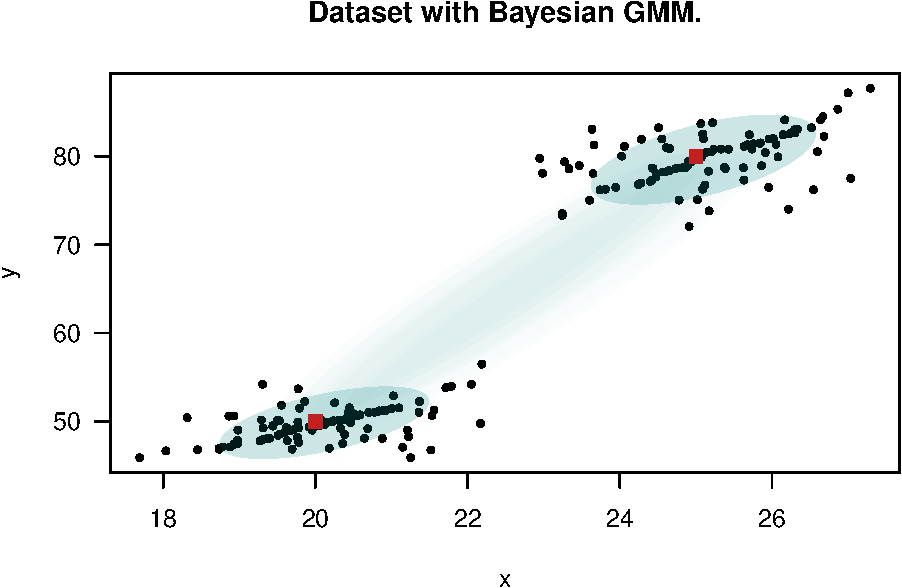
\includegraphics{mclust_sim_files/figure-latex/unnamed-chunk-7-1.pdf}

In conclusion, even though the variational Bayesian implementation did
fit up to 10 clusters (with covariances fully varying) the two correct
clusters were recovered with each cluster being assigned a weight close
to .5 (and all remaining eight spurious clusters were assigned weights
virtually equal to 0).


\end{document}
